\documentclass{article}
\usepackage{graphicx}

\begin{document}

\title{Dokumentation S-Wert}
\author{Honors-Projekt (Fabian Böhm, Alexander Puchta), Gerit Wagner}

\maketitle

\begin{abstract}
The abstract text goes here.
\end{abstract}

\section{Introduction}
Here is the text of your introduction.

\begin{equation}
    \label{simple_equation}
    \alpha = \sqrt{ \beta }
\end{equation}

\subsection{Subsection Heading Here}
Write your subsection text here.

\begin{figure}
    \centering
    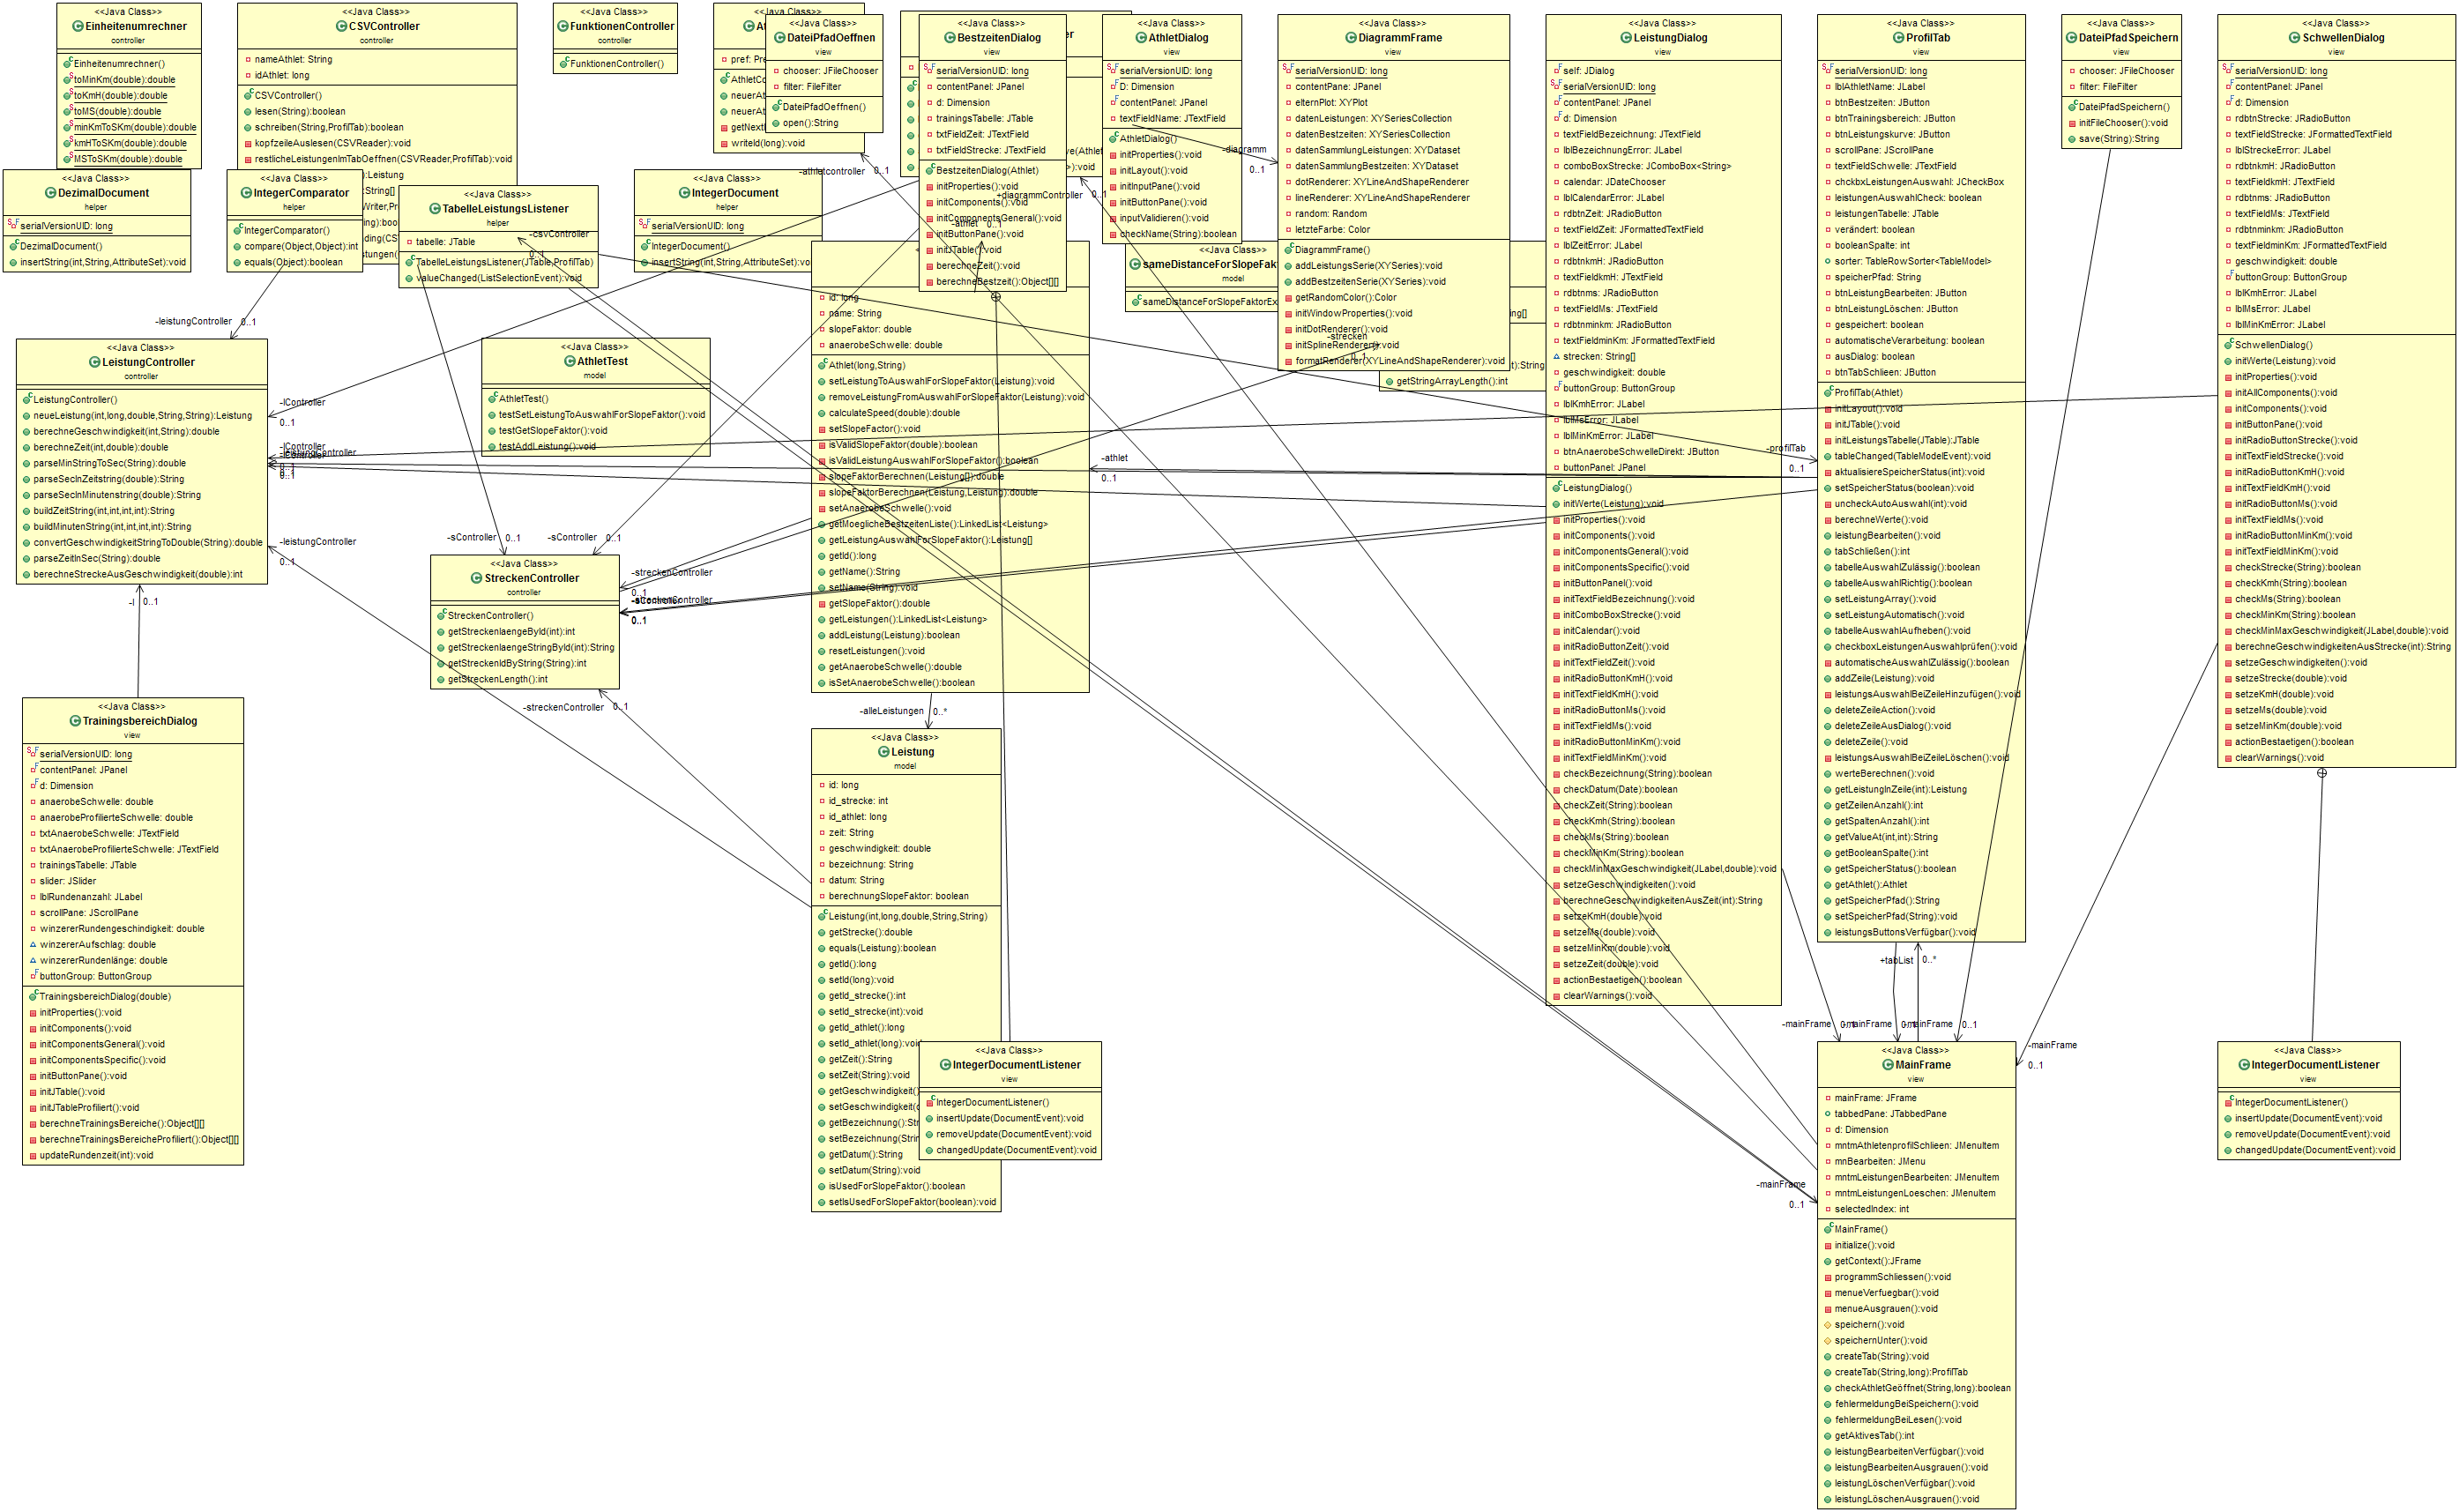
\includegraphics[width=6.0in]{../_diagrams/classes.png}
    \caption{Klassendiagramm}
    \label{classes}
\end{figure}

\begin{figure}
    \centering
    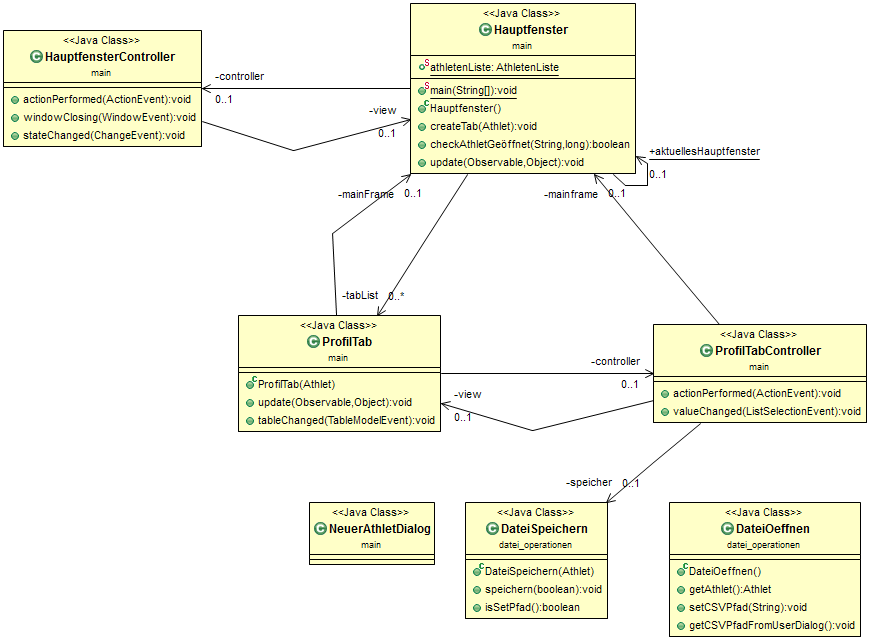
\includegraphics[width=6.0in]{../_diagrams/Main.png}
    \caption{Hauptfenster}
    \label{main}
\end{figure}


\begin{figure}
    \centering
    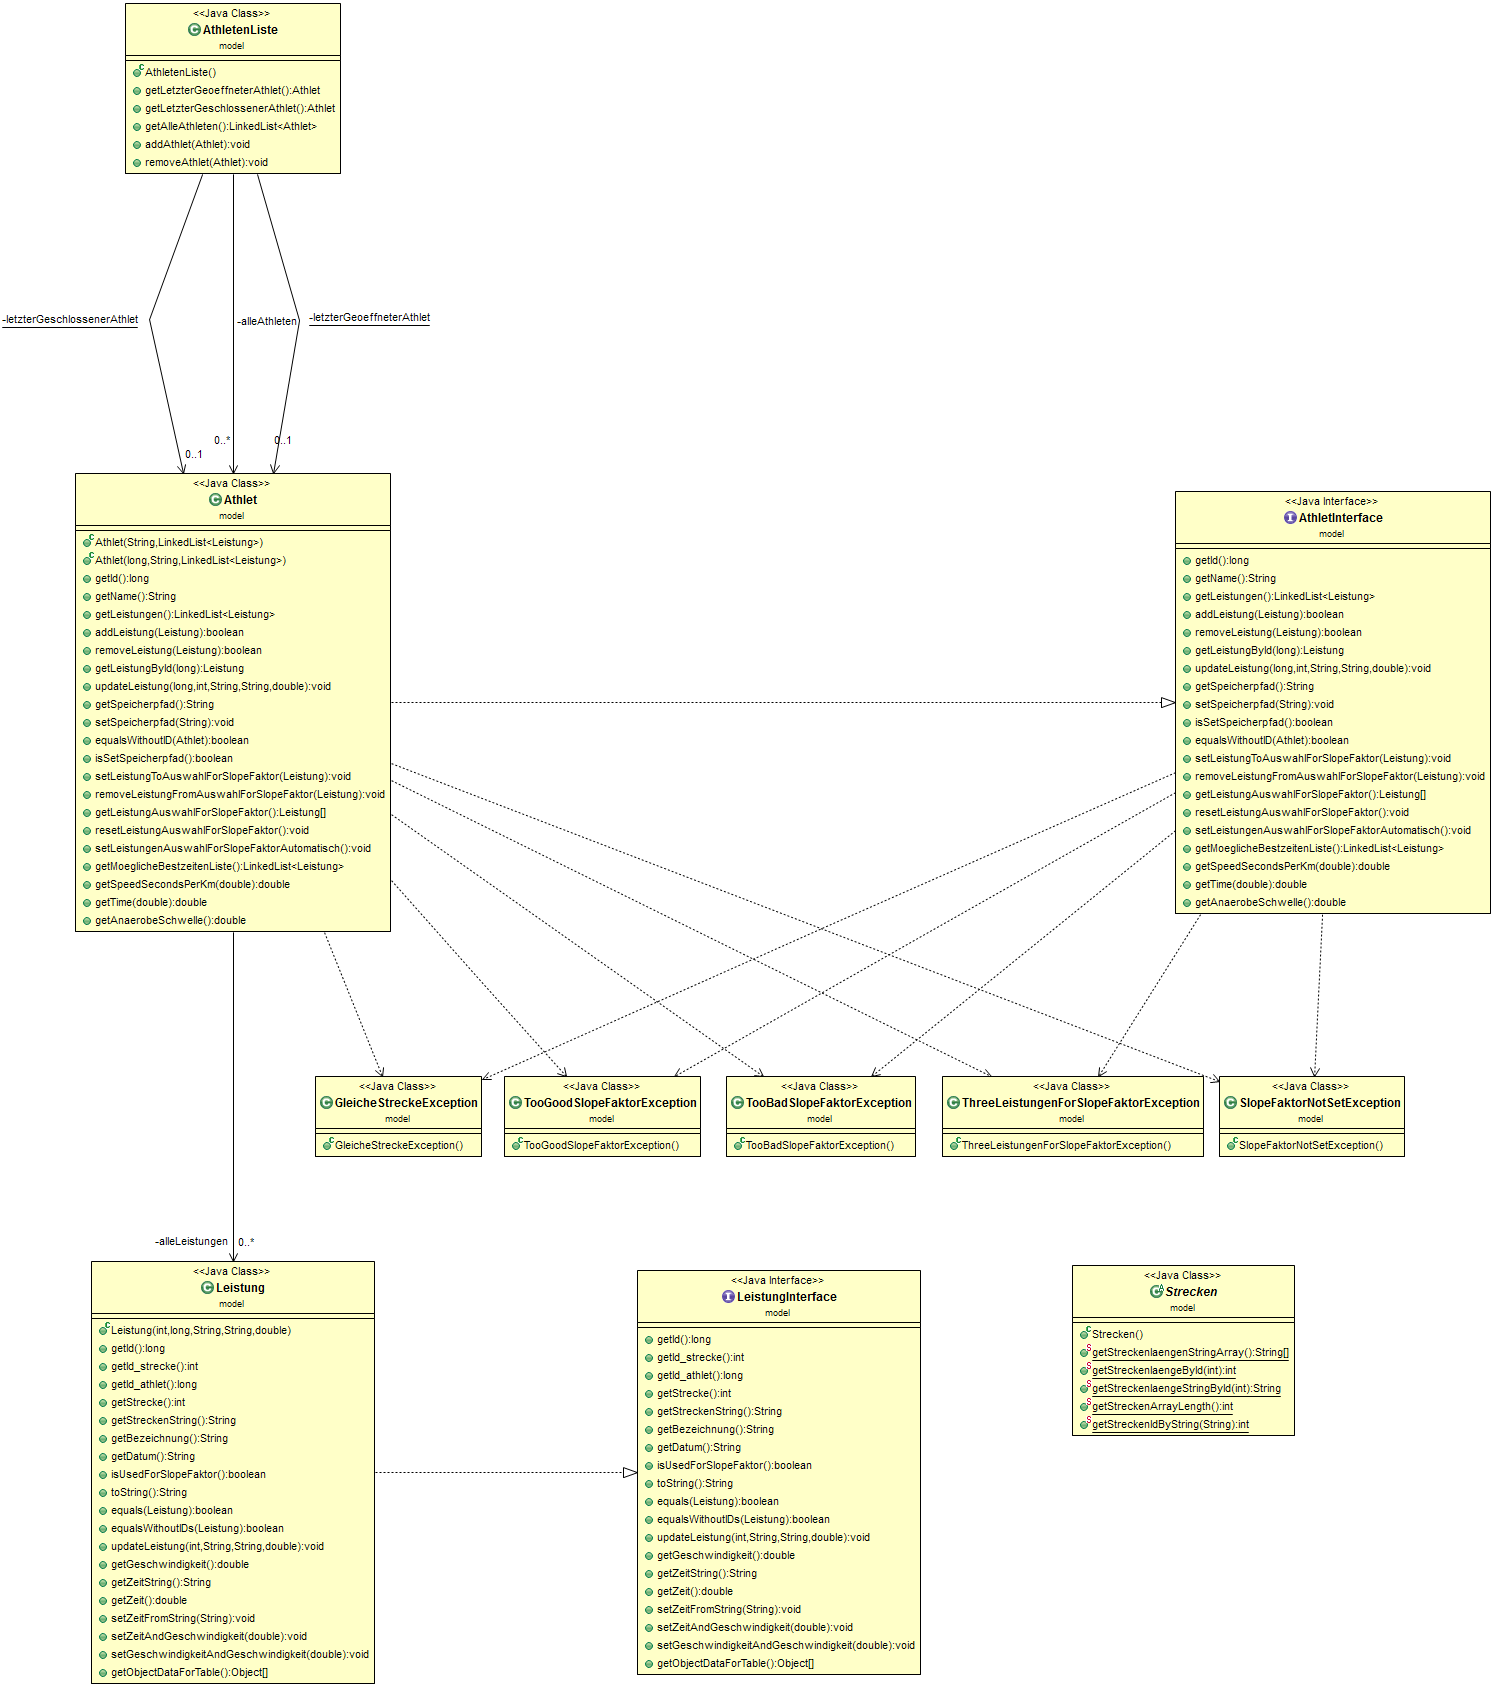
\includegraphics[width=6.0in]{../_diagrams/model.png}
    \caption{Datenmodell}
    \label{model}
\end{figure}

\begin{figure}
    \centering
    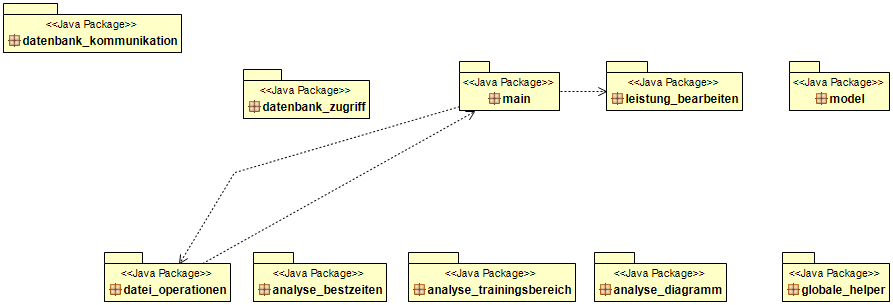
\includegraphics[width=6.0in]{../_diagrams/packages.png}
    \caption{Packete}
    \label{packages}
\end{figure}


\section{Conclusion}
Write your conclusion here.

\end{document}s